\documentclass[11pt]{article}
\usepackage[a4paper,margin=1in]{geometry}
\usepackage[T1]{fontenc}
\usepackage[utf8]{inputenc}
\usepackage{lmodern}
\usepackage{microtype}
\usepackage{amsmath,amssymb,amsthm,mathtools}
\usepackage{booktabs,tabularx,array}
\usepackage{graphicx}
\usepackage{enumitem}
\usepackage{xcolor}
\usepackage[numbers,sort&compress]{natbib}
\usepackage[colorlinks=true,linkcolor=blue!50!black,citecolor=blue!50!black,urlcolor=blue!50!black]{hyperref}
\usepackage[capitalise,noabbrev]{cleveref}

\newtheorem{definition}{Definition}
\newtheorem{proposition}{Proposition}
\newtheorem{corollary}{Corollary}
\theoremstyle{remark}
\newtheorem{remark}{Remark}

\newcommand{\R}{\mathbb{R}}
\newcommand{\E}{\mathbb{E}}
\newcommand{\cK}{\mathcal{K}}
\newcommand{\cR}{\mathcal{R}}
\newcommand{\cT}{\mathcal{T}}
\newcommand{\cN}{\mathcal{N}}
\newcommand{\Cc}{C_{L}}
\newcommand{\Cb}{C_{R}}
\newcommand{\ind}{\mathbf{1}}
\DeclareMathOperator*{\argmin}{arg\,min}

\title{\textbf{Learning Amortization}\\[2pt]
\large Measuring Whether Learning Makes Future Learning Cheaper}
\author{James Jackson\\
\small\url{https://github.com/jacksonjp0311-gif/learning-amortization}}
\date{Working paper v0.1 --- November 2026}

\begin{document}
\maketitle

\begin{abstract}
A learning system that accumulates knowledge is not necessarily a system that gets better at learning.
We make the distinction measurable.
\emph{Learning amortization} compares the \emph{total} cost a continual learner pays to reach a fixed accuracy target on every task of a sequence with the cost paid by a reference learner on the same sequence:
$A_n = 1 - C_{\text{continual}}(n)/C_{\text{reference}}(n)$.
Costs are charged over the whole lifecycle of what is learned: acquisition, verification, storage, retrieval, maintenance and execution, plus any one-time setup.
We give formal definitions and prove the basic properties of the metric: its range and sign, unit invariance (and the precise sense in which it is \emph{not} invariant), an exact weighted-average form, an additive decomposition into cost components, its asymptotic limit and a closed-form break-even point.
We show that the AUC-based forward-transfer metric of Continual World is exactly an amortization ratio whose cost is training steps averaged over all accuracy thresholds, which places the proposal inside existing transfer metrics instead of beside them.
We separate first-order amortization (past learning pays for future learning) from second-order evidence of learning to learn (the savings themselves grow with experience), specify paired-seed estimators, confidence intervals, exact tests and censoring bounds, and list the controls and pitfalls that decide whether a positive $A_n$ means anything.
A small open-source reference implementation reproduces every quantity, and a clearly labelled synthetic example shows the metric detecting both genuine amortization and the classical ``utility problem'' in which a growing library makes learning \emph{more} expensive.
The motivating application is PacketLM, a non-transformer sparse-binary learner; this paper reports \emph{no} PacketLM results and gives only a planned evaluation protocol.
\end{abstract}

\section{Introduction}\label{sec:intro}

The central question behind this paper is simple to state: \emph{does a system become better at learning as a consequence of having learned?}
Two easier questions are often answered in its place.
The first is whether the system knows more after training, which any memory satisfies.
The second is whether it is more accurate on a new task straight away (zero-shot forward transfer), which can be bought with an expensive lookup or a large pre-built library whose cost is never charged.

We argue that the right currency for the central question is \emph{cost at matched accuracy}, summed over everything the system has to do to make prior learning usable.
Speedup-learning research found decades ago that learned macro-operators, explanation-based rules and chunks can make a problem solver slower, because matching and maintaining a growing store costs more than it saves \citep{minton1990quantitative,tambe1990expensive}.
Modern library-learning systems \citep{ellis2021dreamcoder,bowers2023stitch,grand2024lilo} and continual learners face the same trade-off.
A metric that ignores storage, retrieval and maintenance can report progress when there is none.

\paragraph{Contributions.}
This is a measurement paper; it proposes no learning algorithm and makes no empirical claim about any real system.
\begin{enumerate}[leftmargin=*,itemsep=1pt]
\item A \textbf{full-lifecycle cost functional} with an explicit accuracy-matching rule (cost-to-target), declared prices and an attribution rule for costs between tasks (\cref{sec:setup}).
\item The \textbf{learning-amortization} family: cumulative $A_n$, marginal $a_i$, asymptotic $A_\infty$ and break-even $n^\star$, with proofs of their properties (\cref{sec:props}).
\item An \textbf{exact link to forward transfer}: Continual World's FT metric is an amortization ratio over training steps averaged across accuracy thresholds (\cref{prop:ft}).
\item A separation of \textbf{first-order amortization from second-order learning to learn}, via novelty stratification, fork-and-discard probe curves and trend tests (\cref{sec:l2l}).
\item An \textbf{estimation and control protocol} with paired seeds, intervals, exact tests and censoring bounds (\cref{sec:stats,sec:controls,sec:pitfalls}), and a \textbf{reference implementation} with a synthetic worked example (\cref{sec:toy}).
\end{enumerate}

\section{Related work and novelty assessment}\label{sec:related}

\paragraph{Learning to learn and meta-learning.}
The idea that experience with earlier tasks should improve learning of later ones is old and well developed.
It appears in the edited volume of \citet{thrun1998learning}, in multitask learning \citep{caruana1997multitask}, in Baxter's theory of inductive-bias learning \citep{baxter2000model}, and in modern meta-learning \citep{finn2017maml,hospedales2022meta}.
These works mostly measure gains in accuracy or sample efficiency on new tasks; they rarely charge the cost of keeping and consulting what was learned.

\paragraph{Continual-learning metrics.}
\citet{lopezpaz2017gem} define backward transfer (BWT) and forward transfer (FWT) from an accuracy matrix $R_{j,i}$, the test accuracy on task $i$ after training on task $j$.
FWT measures zero-shot accuracy on task $i$ just before it is trained, relative to a random-initialisation baseline.
It is an accuracy quantity and carries no cost.
\citet{diazrodriguez2018dont} add efficiency criteria, including model-size efficiency, sample-storage efficiency and computational efficiency, and combine them with accuracy-based ones in a weighted score.
That work is the closest prior art we found for charging resources in continual learning. As far as we can tell, it does not define cost at matched accuracy or a sequence-level savings ratio.
\citet{chaudhry2018rwalk} introduce intransigence (inability to learn new tasks), and \citet{chaudhry2019agem} introduce the learning-curve area (LCA) as a measure of how quickly a learner acquires new tasks.
\citet{wolczyk2021continual} measure forward transfer as the normalised area between a continual learner's training curve and a from-scratch reference; \cref{prop:ft} shows that this is a special case of the ratio studied here.
\citet{veniat2021efficient} probe several kinds of transfer and report them together with how fast the model grows in size.
\citet{chen2018lifelong} survey lifelong learning more broadly.

\paragraph{Transfer metrics in reinforcement learning.}
\citet{taylor2009transfer} list jumpstart, asymptotic performance, total reward, the transfer ratio and \emph{time to threshold}.
Time to threshold is exactly a per-task cost-to-target when cost is measured in samples, and the transfer ratio is an area ratio.
Our per-task quantity $a_i$ (\cref{def:marg}) generalises time-to-threshold reduction to a multi-component cost.

\paragraph{Speedup learning and the utility problem.}
Learned macro-operators \citep{fikes1972learning}, explanation-based generalisation \citep{mitchell1986ebg} and Soar's chunking \citep{laird1986chunking} all aim to make future problem solving cheaper.
\citet{minton1990quantitative} measured the utility of a learned control rule as its average savings times its application frequency minus its average match cost, and showed that unrestricted learning can slow the solver down.
\citet{tambe1990expensive} traced the same effect to expensive chunks.
Our component decomposition (\cref{prop:decomp}) is the sequence-level analogue of Minton's utility, extended to storage, maintenance and verification.

\paragraph{Library learning.}
DreamCoder \citep{ellis2021dreamcoder} grows a library of reusable functions and a recognition model that guides search, and reports that solving more tasks makes later tasks easier to solve.
Stitch \citep{bowers2023stitch} makes library compression far faster, and LILO \citep{grand2024lilo} combines LLM-guided synthesis with Stitch compression and automatic documentation.
These systems are the natural home for amortization measurements, but their reported metrics are mostly tasks solved and search time under a budget, without a full-lifecycle cost accounting at matched accuracy.

\paragraph{Amortized inference and ``amortised learning''.}
In probabilistic inference, amortization means reusing past computation so that future inferences are cheaper.
\citet{gershman2014amortized} argue that people cache and reuse sub-inferences.
\citet{wenliang2020amortised} use the name \emph{amortised learning} for a wake-sleep method that learns to predict maximum-likelihood parameter updates.
These usages are close in spirit, since earlier computation pays for later computation, but they name algorithms, not a cross-task evaluation metric.
To avoid confusion, we always say \emph{learning amortization} and always mean the metric $A_n$.

\paragraph{Efficiency accounting.}
\citet{schwartz2020green} argue for reporting the computational price of results.
\citet{hernandez2020measuring} measure algorithmic progress as the training compute needed to reach a \emph{fixed} performance level (AlexNet-level ImageNet accuracy), which is the same cost-at-matched-accuracy principle we use.
\citet{dehghani2022efficiency} show that different cost indicators (FLOPs, parameters, throughput) can rank models differently, which motivates our per-resource reporting rule (\cref{prop:basic}(iii)).
\citet{chollet2019measure} defines intelligence as skill-acquisition efficiency relative to priors and experience.
$A_n$ is a much narrower, operational quantity, but it shares the view that efficiency of acquisition, not skill alone, is what should be measured.

\paragraph{Novelty assessment.}
We searched for the phrase ``learning amortization'' and for metrics that combine cost-at-matched-accuracy, a sequence-level savings ratio and full lifecycle costs.
We found no established metric under this name.
The ingredients are not new: time-to-threshold \citep{taylor2009transfer}, area-based forward transfer \citep{wolczyk2021continual}, resource-aware continual-learning criteria \citep{diazrodriguez2018dont}, compute to a fixed performance level \citep{hernandez2020measuring}, and the utility analysis of speedup learning \citep{minton1990quantitative}.
Our contribution is therefore a \emph{synthesis and a protocol}.
It has one definition that charges every lifecycle cost at matched accuracy, proofs of the properties needed to interpret it, an exact reduction showing how an established forward-transfer metric fits inside it, and a control and statistics protocol aimed at separating learning to learn from accumulation.
We make no stronger novelty claim.

\section{Formal setup}\label{sec:setup}

\begin{definition}[Task sequence and protocol]\label{def:protocol}
A seed $s$ determines, through a fixed generator, a task sequence $\cT^{(s)} = (T_1,\dots,T_N)$.
Each task $T_i$ provides an interaction source (examples, teaching turns, oracle queries) and a \emph{sealed} evaluation set $E_i$ that no learner reads.
A learner $L$ has a state $M$ (memory, library, parameters).
A \emph{continual} learner starts task $i$ from the state $M_{i-1}$ left by task $i-1$, starting from an initial state $M_0$.
A \emph{reference} learner $R$ runs on the same $\cT^{(s)}$ under a protocol specified in \cref{sec:controls}; the default reference resets its state to $M_0$ before every task.
\end{definition}

\begin{definition}[Cost functional]\label{def:cost}
Let $\cK = \{\mathrm{acq},\mathrm{ver},\mathrm{sto},\mathrm{ret},\mathrm{mnt},\mathrm{exe}\}$ be the cost components and $\cR$ a finite set of measured resources (e.g.\ primitive operations, CPU-seconds, byte-seconds of storage, oracle queries, teacher turns).
For task index $i\in\{0,\dots,N\}$, component $k$ and resource $r$, let $q_{i,k,r}\ge 0$ be the measured amount.
Index $i=0$ collects one-time costs paid before $T_1$.
Given a price vector $w\in\R_{\ge 0}^{\cR}$ \emph{declared before the experiment},
\begin{equation}\label{eq:cost}
c_{i,k} = \sum_{r\in\cR} w_r\, q_{i,k,r}, \qquad c_i = \sum_{k\in\cK} c_{i,k}.
\end{equation}
\emph{Attribution rule.} Every cost incurred from the moment the learner is ready to accept $T_i$ until the moment it is ready to accept $T_{i+1}$ is charged to $i$; costs before $T_1$ are charged to $0$.
Thus post-task consolidation, deduplication and checkpointing are charged to the task that triggered them.
Experimenter-side evaluation on $E_i$ is not charged.
The learner's own execution to produce answers for $E_i$ is charged as $c_{i,\mathrm{exe}}$.
\end{definition}

The components have the following meanings.
\emph{Acquisition} covers search, candidate generation, parameter updates and interaction with the teacher or oracle.
\emph{Verification} covers checking candidates against evidence, consistency checks and re-verification after corrections or retractions.
\emph{Storage} is the holding cost of the state, measured in a resource such as byte-seconds, $\int |M(t)|\,dt$ over the task's interval, so a library that is never used still costs something.
\emph{Retrieval} covers indexing, lookup and matching of stored items, which is Minton's match cost.
\emph{Maintenance} covers consolidation, compression, deduplication, dependency propagation, invalidation and checkpoint I/O.
\emph{Execution} is running the acquired capability.

\begin{definition}[Cost-to-target]\label{def:ctt}
Fix, before the experiment, an accuracy target $\alpha_i\in(0,1]$ and a budget $B_i>0$ for every task.
Let $\mathrm{acc}_i(L,t)$ be the accuracy on $E_i$ of the hypothesis $L$ has committed to after spending cost $t$ on $T_i$.
The learning phase of $T_i$ ends at a time $\tau_i(L)$ defined in one of two ways, declared in advance:
\begin{itemize}[itemsep=1pt]
\item \emph{anytime learners}: $\tau_i(L) = \min\bigl(B_i,\ \inf\{t\ge 0: \mathrm{acc}_i(L,t)\ge \alpha_i\}\bigr)$, where the experimenter evaluates checkpoints on $E_i$ without feeding any result back to the learner;
\item \emph{self-stopping learners}: $\tau_i(L)=\min(B_i,\sigma_i)$, where $\sigma_i$ is the moment the learner commits by its own criterion.
\end{itemize}
$c_i(L)$ is the total cost charged to $i$ by \cref{def:cost}: the cost up to $\tau_i$ plus the post-task costs (consolidation, maintenance, execution on $E_i$) the attribution rule assigns to $i$.
The censoring indicator is $\delta_i(L)=\ind[\mathrm{acc}_i(L,\tau_i)<\alpha_i]$.
\end{definition}

\begin{remark}[Accuracy matching]
A task's cost counts as \emph{matched} for an arm only if $\delta_i=0$.
Cost-to-target makes accuracies comparable by construction.
The alternative, a fixed budget with an equivalence test on accuracy (e.g.\ two one-sided tests with a declared margin), is also valid but must be declared in advance.
Comparing costs at different accuracies is not valid.
\end{remark}

\begin{definition}[Cumulative cost]\label{def:cum}
$C_L(n) = \sum_{i=0}^{n} c_i(L)$ for $n=0,\dots,N$.
\end{definition}

\begin{definition}[Learning amortization]\label{def:A}
For a learner $L$, a reference $R$ and a horizon $1\le n\le N$ with $C_R(n)>0$,
\begin{equation}\label{eq:A}
\boxed{\;A_n(L\,\|\,R) \;=\; 1-\frac{C_L(n)}{C_R(n)}\;}
\end{equation}
We write $A_n$ when $L$ and $R$ are clear from context.
$A_n>0$ means $L$ paid less than $R$ in total to reach the same targets on the first $n$ tasks.
\end{definition}

\begin{definition}[Marginal and asymptotic amortization]\label{def:marg}
For $i\ge 1$ with $c_i(R)>0$, the marginal amortization is $a_i = 1 - c_i(L)/c_i(R)$, and we set $a_0 = 1-c_0(L)/c_0(R)$ when $c_0(R)>0$.
The asymptotic amortization is $A_\infty = \lim_{n\to\infty} A_n$ when the limit exists.
The tail-window estimator with window $k$ is
\[
A^{(k)}_N = 1-\frac{\sum_{i=N-k+1}^{N} c_i(L)}{\sum_{i=N-k+1}^{N} c_i(R)}.
\]
\end{definition}

\begin{definition}[Break-even point]\label{def:be}
$n^\star = \min\{n\in\{1,\dots,N\}: A_m>0 \text{ for all } m\in\{n,\dots,N\}\}$, and $n^\star$ is undefined if $A_N\le 0$.
Requiring positivity on the rest of the horizon prevents a temporary crossing from being reported as break-even.
\end{definition}

\section{Properties}\label{sec:props}

All proofs are short and given inline. Each property has an executable check in \texttt{tests/}.

\begin{proposition}[Basic properties]\label{prop:basic}
Let $C_R(n)>0$.
\begin{enumerate}[label=(\roman*),itemsep=1pt]
\item \emph{Range and sign.} $A_n\le 1$, with equality if and only if $C_L(n)=0$, and $A_n$ is unbounded below. $A_n>0$, $=0$ or $<0$ according as $C_L(n)<$, $=$ or $>C_R(n)$.
\item \emph{Unit invariance.} Replacing $w$ by $\lambda w$ for any $\lambda>0$ leaves $A_n$ unchanged. In particular, with a single resource, $A_n$ does not depend on the unit.
\item \emph{No invariance to relative prices.} With two or more resources, changing the \emph{relative} prices can change the sign of $A_n$. Results must therefore be reported per resource as well as for the declared $w$.
\item \emph{Log form and asymmetry.} With $\ell_n = \log C_R(n) - \log C_L(n)$ (for $C_L(n)>0$), $A_n = 1-e^{-\ell_n}$. Moreover $\ell_n(R\|L)=-\ell_n(L\|R)$, whereas $A_n(R\|L) = -A_n(L\|R)/(1-A_n(L\|R))$.
\item \emph{Weighted average.} Let $P=\{i\le n: c_i(R)>0\}$ and $Z=\{i\le n: c_i(R)=0\}$. Then
\begin{equation}\label{eq:wavg}
A_n = \sum_{i\in P}\omega_i\, a_i \;-\; \sum_{i\in Z}\frac{c_i(L)}{C_R(n)},\qquad \omega_i = \frac{c_i(R)}{C_R(n)},\quad \sum_{i\in P}\omega_i = 1 .
\end{equation}
In the common case $c_0(R)=0$ (a reference with no setup), the learner's whole setup cost enters through the second sum as a pure penalty. If $Z=\varnothing$, then $A_n$ is exactly the $\omega$-weighted mean of the marginal amortizations.
\end{enumerate}
\end{proposition}
\begin{proof}
(i) Costs are non-negative, so $C_L(n)/C_R(n)\ge 0$, and the ratio is $0$ only when $C_L(n)=0$. Letting $C_L(n)\to\infty$ shows that $A_n$ is unbounded below. The sign statement follows by rearranging the definition.
(ii) Both cumulative costs are linear in $w$ by \eqref{eq:cost}, so the common factor $\lambda$ cancels.
(iii) Consider one task, $c_0=0$ and two resources (operations and memory). Let $L$ use $(1,10)$ and $R$ use $(10,0)$. With prices $(1,0.1)$, $A_1 = 1-2/10 = 0.8$. With prices $(1,10)$, $A_1 = 1-101/10 = -9.1$.
(iv) $C_L/C_R = e^{-\ell_n}$. Swapping the arms gives $1-C_R/C_L = 1-1/(1-A_n)$.
(v) $1-\frac{C_L(n)}{C_R(n)} = \sum_{i\le n} \frac{c_i(R)-c_i(L)}{C_R(n)}$. For $i\in P$ the summand equals $\frac{c_i(R)}{C_R(n)}\bigl(1-\frac{c_i(L)}{c_i(R)}\bigr)=\omega_i a_i$, and for $i\in Z$ it equals $-c_i(L)/C_R(n)$. Finally $\sum_{i\in P}c_i(R)=C_R(n)$.
\end{proof}

Item (v) shows that cumulative amortization weights each task by its \emph{reference} cost, so hard tasks dominate.
This is deliberate, because it reports savings in the currency actually spent.
An unweighted mean of $a_i$, as used for FT by \citet{wolczyk2021continual}, answers a different question and should be labelled as such.
Because of (iv), averages of $A$ across seeds should be taken on the $\ell$ scale or as ratios of sums, never as unweighted arithmetic means of per-seed $A$ values.

\begin{proposition}[Component decomposition]\label{prop:decomp}
Write $C_{L,k}(n)=\sum_{i\le n}c_{i,k}(L)$ and similarly for $R$. Then
\begin{equation}\label{eq:decomp}
A_n = \sum_{k\in\cK} D_{n,k},\qquad D_{n,k} = \frac{C_{R,k}(n)-C_{L,k}(n)}{C_R(n)} .
\end{equation}
\end{proposition}
\begin{proof}
$C_R(n)-C_L(n) = \sum_k \bigl(C_{R,k}(n)-C_{L,k}(n)\bigr)$. Divide by $C_R(n)$.
\end{proof}

\begin{corollary}[Utility condition]\label{cor:utility}
Partition $\cK$ into components on which $L$ saves ($D_{n,k}\ge 0$) and overheads ($D_{n,k}<0$). Then $A_n>0$ if and only if the total savings exceed the total overheads:
\[
\sum_{k: D_{n,k}\ge 0}\bigl(C_{R,k}-C_{L,k}\bigr) \;>\; \sum_{k: D_{n,k}<0}\bigl(C_{L,k}-C_{R,k}\bigr).
\]
A memoryless reference typically has $C_{R,\mathrm{ret}}=C_{R,\mathrm{mnt}}=0$, so for a library learner retrieval and maintenance enter only as overheads. This is Minton's utility problem \citep{minton1990quantitative} at the scale of a whole sequence.
\end{corollary}

\begin{proposition}[Asymptotic limit]\label{prop:asym}
Suppose $c_0(L),c_0(R)<\infty$ and the per-task averages converge: $\frac1n\sum_{i=1}^n c_i(L)\to\gamma_L$ and $\frac1n\sum_{i=1}^n c_i(R)\to\gamma_R>0$. Then
\[
A_\infty = \lim_{n\to\infty}A_n = 1-\frac{\gamma_L}{\gamma_R}.
\]
\end{proposition}
\begin{proof}
$\frac{C_L(n)}{C_R(n)} = \frac{c_0(L)/n + \frac1n\sum_{i=1}^n c_i(L)}{c_0(R)/n+\frac1n\sum_{i=1}^n c_i(R)}\to\frac{\gamma_L}{\gamma_R}$, since the denominator tends to $\gamma_R>0$.
\end{proof}
One-time costs vanish from $A_\infty$. A system with an enormous pre-built library can therefore look excellent asymptotically while never repaying its setup within any realistic horizon.
$A_\infty$ or $A^{(k)}_N$ must always be reported together with $A_N$ at the actual horizon and with $n^\star$.

\begin{proposition}[Break-even under constant costs]\label{prop:be}
Let $c_0(L)=c_0(R)+\Delta_0$ with $c_0(R)\ge 0$ and $c_0(L)\ge 0$, and for $i\ge1$ let $c_i(R)=\gamma>0$ and $c_i(L)=\gamma-\delta$ with $0<\delta\le\gamma$. Then
\[
A_n = \frac{n\delta-\Delta_0}{c_0(R)+n\gamma},
\]
which is non-decreasing in $n$ when $\Delta_0\ge 0$ and tends to $\delta/\gamma$. Consequently $n^\star = \lfloor \Delta_0/\delta\rfloor+1$ if $\Delta_0\ge 0$ and $n^\star=1$ if $\Delta_0<0$ (for $N\ge n^\star$).
\end{proposition}
\begin{proof}
$1-\frac{c_0(R)+\Delta_0+n(\gamma-\delta)}{c_0(R)+n\gamma} = \frac{n\delta-\Delta_0}{c_0(R)+n\gamma}$. Its derivative in $n$ has the sign of $\delta c_0(R)+\gamma\Delta_0$, which is $\ge 0$ when $\Delta_0\ge0$. So when $\Delta_0\ge 0$, $A_n>0$ exactly when $n>\Delta_0/\delta$ and positivity then persists, giving the first integer above $\Delta_0/\delta$. When $\Delta_0<0$ the numerator is positive for all $n\ge1$.
\end{proof}

\subsection{Relation to forward transfer}\label{sec:ft}

Let a learning curve on a task be $p_0,\dots,p_{D-1}\in[0,1]$, the performance after $k$ units of training cost, with budget $D$.
Define the first-hit cost $t(\alpha)=\min\{k: p_k\ge\alpha\}$ (or $D$ if the target is never reached), the normalised area $\mathrm{AUC}=\frac1D\sum_k p_k$, and
\[
I(p) = \int_0^1 \min\bigl(t(\alpha),D\bigr)\,d\alpha ,
\]
the cost-to-target averaged uniformly over all targets $\alpha$ and censored at the budget.

\begin{proposition}[Forward transfer is an amortization ratio]\label{prop:ft}
If $p$ is non-decreasing, then (i) $\mathrm{AUC} = 1 - I(p)/D$. Hence (ii), for non-decreasing $p$ (continual) and $p^b$ (reference) with $\mathrm{AUC}^b<1$, the Continual World forward transfer \citep{wolczyk2021continual} satisfies
\[
\mathrm{FT} = \frac{\mathrm{AUC}-\mathrm{AUC}^b}{1-\mathrm{AUC}^b} = 1-\frac{I(p)}{I(p^b)} .
\]
\end{proposition}
\begin{proof}
(i) $p_k = \int_0^1 \ind[p_k\ge\alpha]\,d\alpha$, so $\sum_k p_k = \int_0^1 \bigl|\{k: p_k\ge\alpha\}\bigr|\,d\alpha$. For a non-decreasing curve, $\{k:p_k\ge\alpha\}=\{t(\alpha),\dots,D-1\}$, which has $D-\min(t(\alpha),D)$ elements. Dividing by $D$ gives the claim.
(ii) By (i), $\mathrm{AUC}-\mathrm{AUC}^b = (I(p^b)-I(p))/D$ and $1-\mathrm{AUC}^b = I(p^b)/D>0$.
\end{proof}
The same proof works in continuous time, which is the form used by \citet{wolczyk2021continual}. For a non-decreasing $p:[0,\Delta]\to[0,1]$, Tonelli's theorem gives $\int_0^\Delta p(t)\,dt=\int_0^1 \bigl(\Delta-\min(t(\alpha),\Delta)\bigr)\,d\alpha$ with $t(\alpha)=\inf\{t:p(t)\ge\alpha\}$.
FT is thus learning amortization for a single task in which cost is training steps only, the target is averaged over $[0,1]$ instead of fixed, costs are censored at the budget, and tasks are then averaged without weights.
$A_n$ keeps the ratio form but fixes a declared target, charges every lifecycle component and aggregates by cost.
For curves that rise and then collapse, AUC and $I$ disagree.
The test suite includes a counterexample, so monotonicity (or a running maximum) must be stated whenever this correspondence is used.
By contrast, GEM's FWT \citep{lopezpaz2017gem} is a zero-shot accuracy difference.
Positive FWT is neither necessary nor sufficient for $A_n>0$: a learner can be accurate zero-shot only through an expensive retrieval, or have zero zero-shot accuracy and still learn each new task cheaply.

\section{First-order amortization versus learning to learn}\label{sec:l2l}

\subsection{Two different claims}
$A_n>0$ is a \emph{first-order} claim: what was learned earlier pays for part of what is learned later.
That can happen without the learning process improving at all, for example when later tasks repeat earlier ones and the learner retrieves stored answers.
The stronger, \emph{second-order} claim is that the learner's capacity to acquire genuinely new capabilities grows with experience.
The three instruments below target the second claim.

\begin{definition}[Novelty-stratified amortization]\label{def:novel}
Before running, the generator labels each task \emph{novel} or \emph{familiar} by a criterion that does not depend on outcomes. A task is novel, for instance, if its solution is not equivalent to any solution of an earlier task and it uses relations or entities withheld from earlier tasks.
With $\cN$ the novel tasks among the first $n$,
\[
A_n^{\mathrm{nov}} = 1-\frac{c_0(L)+\sum_{i\in\cN}c_i(L)}{c_0(R)+\sum_{i\in\cN}c_i(R)}.
\]
Both arms' full setup costs are kept. When $c_0(L)\ge c_0(R)$, the usual case for a learner that ships with or builds a library, this charges the whole extra setup to the novel tasks and is conservative for the learner.
\end{definition}

\begin{definition}[Fork-and-discard probe curve]\label{def:probe}
Fix sealed probe tasks $P_1,\dots,P_m$ that never enter any learner's state.
After task $k$ of the sequence, copy the state $M_k$, solve each probe from the copy, record the cost-to-target $c_{P_j}(M_k)$, then discard the copy.
The probe amortization is
\[
\Pi(k) = 1-\frac{\sum_j c_{P_j}(M_k)}{\sum_j c_{P_j}(M_0)} .
\]
\end{definition}
Because the probes are discarded, $\Pi(k)$ measures how cheap \emph{new} learning has become at stage $k$ without contaminating the sequence.
Evidence for learning to learn is a $\Pi(k)$ that rises with $k$ on probes that are novel by the criterion of \cref{def:novel}.

\subsection{Trend test}\label{sec:trend}
Let $\ell_{s,i} = \log c_i^{(s)}(R)-\log c_i^{(s)}(L)$ be the per-task log ratio in seed $s$, and $\bar\ell_i$ its mean over seeds.
The trend $\beta$ is the ordinary least-squares slope of $\bar\ell_i$ on $i$, with a bootstrap interval obtained by resampling seeds.
A positive $\beta$ means the per-task savings grow along the sequence, which is the signature of compounding.
$\beta\approx 0$ with $A_n>0$ means a fixed advantage, for example a useful initial library.
$\beta$ measures growth in \emph{relative} savings. If later tasks are harder for the reference while $L$'s absolute cost stays flat, $\beta>0$ even though $L$'s learning has not accelerated in absolute terms. $\beta$ must therefore be read alongside absolute per-task costs, $\Pi(k)$ and the order-shuffled control.

\section{Estimation and inference}\label{sec:stats}

\subsection{Design}
Run $S$ independent seeds.
Within a seed, every arm sees the same task sequence, the same splits and the same sealed sets, which makes the design \emph{paired}.
Let $X_s = C_L^{(s)}(n)$ and $Y_s = C_R^{(s)}(n)$.
Before running, fix and record the following: $\alpha_i$, $B_i$, $w$, the generator, $S$, $n$, the novelty criterion, the primary comparison and the analysis code version.
Where possible, use deterministic operation counts as the primary cost, and wall-clock time on pinned cores, with repetitions, as a secondary cost.

\subsection{Estimators, intervals and tests}\label{sec:est}
The population quantity is $A_n = 1-\E X/\E Y$, the savings on the total spent by a population of runs. Its plug-in estimator is the ratio of means,
\begin{equation}\label{eq:est}
\hat A_n = 1-\frac{\sum_s X_s}{\sum_s Y_s},
\end{equation}
which is consistent by the strong law of large numbers and continuity of $(x,y)\mapsto 1-x/y$ at $(\E X,\E Y)$ with $\E Y>0$.
The mean of per-seed $A$ values estimates a different quantity, $1-\E[X/Y]$, and is distorted by the asymmetry noted in \cref{prop:basic}(iv). We do not use it.
As a robustness check we also report the geometric form $1-\exp(-\bar\ell)$ with $\bar\ell = \frac1S\sum_s \ell_s$ and $\ell_s=\log Y_s-\log X_s$.

\emph{Delta-method standard error.} With $\hat\rho = \bar X/\bar Y$ and residuals $d_s = X_s-\hat\rho Y_s$ (which sum to zero),
\begin{equation}\label{eq:se}
\widehat{\mathrm{SE}}(\hat A_n) = \frac{1}{\bar Y}\sqrt{\frac{1}{S(S-1)}\sum_{s=1}^S d_s^2 } .
\end{equation}

\emph{Paired bootstrap.} Resample whole seeds with replacement, using the same indices for both arms, recompute \eqref{eq:est}, and report percentile intervals \citep{efron1993bootstrap}.
For small $S$, treat intervals as descriptive and report every per-seed value, following \citet{agarwal2021deep}.

\emph{Exact test.} Under $H_0$, the distribution of $\ell_s$ is symmetric about $0$ (no amortization). The sign-flip permutation test uses $|\bar\ell|$ and enumerates all $2^S$ sign patterns. The smallest attainable two-sided $p$-value is $2/2^S$, so $S\ge 6$ seeds are needed before $p<0.05$ is even possible.
The Wilcoxon signed-rank test on $\ell_s$ is an alternative.
Across several controls, correct for multiplicity (e.g.\ Holm).
On paired designs and the dangers of naive $t$-tests over resampled splits, see \citet{dietterich1998approximate}.

\subsection{Censoring}\label{sec:cens}
A censored task (\cref{def:ctt}) is recorded at the cost actually spent: the budget, or the stopping cost of a committed hypothesis that missed the target. Reaching the target in the same run would have required at least that much, so the recorded cost is a \emph{lower} bound on the true cost-to-target.
\begin{proposition}[Censoring bounds]\label{prop:cens}
Let $\tilde C_L,\tilde C_R$ be the recorded and $C_L\ge\tilde C_L$, $C_R\ge\tilde C_R$ the true cumulative costs.
If only $L$ has censored tasks ($C_R=\tilde C_R$), the recorded $\tilde A_n$ is an \emph{upper} bound on $A_n$ (optimistic).
If only $R$ has censored tasks, $\tilde A_n$ is a \emph{lower} bound (pessimistic).
If both do, the direction is undetermined.
\end{proposition}
\begin{proof}
$A_n$ is decreasing in $C_L$ and increasing in $C_R$ for $C_R>0$.
\end{proof}
Censoring counts per arm must be reported.
Dropping censored tasks from the analysis is selection on the outcome, and is not allowed.

\section{Required controls}\label{sec:controls}

Each control is a reference $R$ in $A_n(L\|R)$ and answers one question. \Cref{tab:controls} lists them.

\begin{table}[ht]
\centering\small
\begin{tabularx}{\linewidth}{>{\raggedright\arraybackslash}p{2.6cm}>{\raggedright\arraybackslash}X>{\raggedright\arraybackslash}X}
\toprule
Control & What changes & What $A_n(L\|\text{control})>0$ shows\\
\midrule
Empty-memory & State reset to $M_0$ before every task & Carried-over state pays for itself (default reference)\\
Frozen & State frozen after a warm-up of $w_0$ tasks & Continued learning helps beyond the initial library (evaluate on tasks after $w_0$)\\
Primitive-only & Acquired procedures disabled; facts kept & Reuse of \emph{procedures}, not only stored facts, drives savings\\
Shuffled-evidence & Same volume of experience with evidence--label pairing permuted & Savings depend on the \emph{content} of experience, not its volume or caching artefacts\\
Symbolic reference & Efficient indexed symbolic implementation of the same tasks & $L$ is competitive in absolute terms, not only against itself\\
Geometry-disabled & Geometric activation and pruning replaced by exhaustive or indexed operations & Savings are attributable to the geometric (Bitwork) mechanism\\
Order-shuffled & Same tasks, randomised order & Savings are not an artefact of a hand-ordered curriculum\\
Exact-repeat cache & Pure memoisation of identical tasks & Upper bound on what caching alone achieves; $L$ must beat it on novel tasks\\
\bottomrule
\end{tabularx}
\caption{Controls. The first six come from the PacketLM qualification plan; the last two are additions recommended here. All arms run the same frozen engine source, identified by its hash.}
\label{tab:controls}
\end{table}

\section{Pitfalls}\label{sec:pitfalls}
\begin{enumerate}[leftmargin=*,itemsep=2pt]
\item \textbf{Cached results mistaken for capability.} Overlapping or repeated tasks give large $A_n$ through retrieval alone. \emph{Mitigation:} use $A_n^{\mathrm{nov}}$, $\Pi(k)$ and the exact-repeat cache control.
\item \textbf{Leakage.} Sealed sets read by the learner, probes written into its state, or a library seeded from evaluation material all invalidate the result. \emph{Mitigation:} hash the sealed sets, use fork-and-discard probes, and log the provenance of every stored item.
\item \textbf{Post-hoc thresholds and prices.} Choosing $\alpha$, $B$ or $w$ after seeing results can manufacture a positive $A_n$. \emph{Mitigation:} pre-register them and report the curve $\alpha\mapsto A_n(\alpha)$ and the per-resource results as sensitivity analyses.
\item \textbf{Unpriced costs.} Omitting storage, retrieval, maintenance, verification or setup hides the utility problem (\cref{cor:utility}). Teacher effort in interactive teaching is a resource and must be counted, for example as teacher turns.
\item \textbf{Developer improvements counted as learning.} Changing engine code between tasks moves cost from the learner to the developer. \emph{Mitigation:} freeze the engine source and run all arms on the same hash.
\item \textbf{Weak references.} A deliberately slow baseline inflates $A_n$. \emph{Mitigation:} include the symbolic reference and report absolute costs.
\item \textbf{Description length mistaken for cost.} A shorter program is not necessarily cheaper to find, verify or run. Measure operations.
\item \textbf{Aggregation errors.} Averaging $A$ values across seeds, or mixing weighted and unweighted task averages, changes the estimand (\cref{prop:basic}(iv)--(v)).
\item \textbf{Dropping failures.} Removing censored tasks or failed seeds is selection on the outcome (\cref{prop:cens}).
\end{enumerate}

\section{Reference implementation and a synthetic worked example}\label{sec:toy}

The package \texttt{amortization/} implements every quantity above. It includes cost logs with declared prices (\cref{def:cost}), $A_n$, $a_i$, $A^{(k)}_N$, $n^\star$, the decomposition \eqref{eq:decomp}, the estimator \eqref{eq:est}, the standard error \eqref{eq:se}, the paired bootstrap, the exact sign-flip test, the trend $\beta$, $A_n^{\mathrm{nov}}$, $\Pi(k)$, and the functions used to check \cref{prop:ft}.
Each proposition has a test.

\paragraph{The example is synthetic.}
The following numbers come from a toy program-search world written for this paper. They say nothing about PacketLM or any other real system.
Inputs are $\mathbb{Z}_{16}$ and there are six fixed primitive maps.
Each task is a hidden map given by 10 training pairs, with 6 sealed test inputs.
A learner enumerates compositions breadth-first up to depth 5, commits to the first one consistent with the training pairs, and succeeds if it is exactly correct on the sealed inputs ($\alpha=1$).
The \emph{base} arm is empty-memory.
The \emph{library} arm stores each correct solution and offers it as an extra building block on later tasks, a much simplified version of DreamCoder's library.
Costs are counted operations, not simulated.
Acquisition is one operation per computed output, verification is one per training comparison, retrieval is one per library fetch, storage is $0.01$ per stored cell per task, maintenance is one per cell compared during deduplication, and execution is one per sealed input.
In the \emph{compositional} curriculum, each target composes two earlier targets or primitives, so reuse is possible.
In the \emph{unrelated} curriculum, targets are independent depth-3 compositions of primitives.
We used $S=20$ seeds, $N=12$ tasks and $10^4$ bootstrap resamples. The run takes about three seconds and is reproduced by \texttt{python examples/synthetic\_toy.py}.

\begin{table}[ht]
\centering\small
\begin{tabular}{lrr}
\toprule
 & Compositional & Unrelated \\
\midrule
$\hat A_{12}$ (ratio of means) & $0.917$ & $-2.261$\\
95\% paired bootstrap CI & $[0.869,\ 0.941]$ & $[-2.539,\ -1.975]$\\
Delta-method SE & $0.017$ & $0.147$\\
Sign-flip $p$ ($10^5$ Monte Carlo draws) & $<10^{-4}$ & $<10^{-4}$\\
Tail window $A^{(4)}_{12}$ (seed-mean costs) & $0.933$ & $-4.306$\\
Break-even $n^\star$ (seed-mean costs) & $2$ & none\\
Trend $\beta$ [95\% CI] & $0.147\ [0.103, 0.193]$ & $-0.137\ [-0.154,-0.119]$\\
Censored tasks, base / library (of 240) & $12$ / $0$ & $1$ / $1$\\
\midrule
$D_{\mathrm{acq}}$ / $D_{\mathrm{ver}}$ & $0.847$ / $0.078$ & $-1.993$ / $-0.140$\\
$D_{\mathrm{ret}}$ / $D_{\mathrm{mnt}}$ / $D_{\mathrm{sto}}$ & $-0.002$ / $-0.005$ / $-0.0001$ & $-0.091$ / $-0.037$ / $-0.0004$\\
\bottomrule
\end{tabular}
\caption{SYNTHETIC toy example (not PacketLM). The component contributions $D_k$ (\cref{prop:decomp}) are computed on seed-mean costs and sum exactly to $\hat A_{12}$ (a ratio of means equals a ratio of seed-mean costs). Execution contributes $0$ in both curricula.}
\label{tab:toy}
\end{table}

\begin{figure}[ht]
\centering
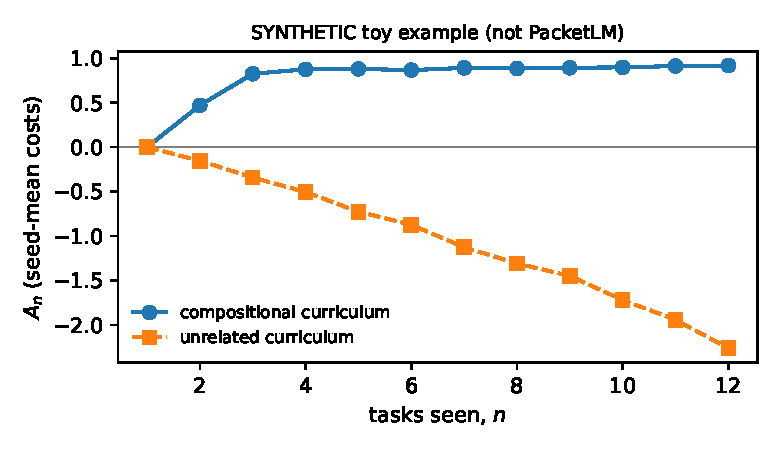
\includegraphics[width=0.62\linewidth]{figures/synthetic_curve.pdf}
\caption{SYNTHETIC. $A_n$ on seed-mean costs for the two curricula. The same library mechanism amortizes strongly when tasks compose and is strongly \emph{negative} when they do not.}
\label{fig:toy}
\end{figure}

\paragraph{Reading the example.}
In the compositional curriculum, $A_{12}$ is large and the trend is positive. The decomposition shows that the savings are almost entirely in acquisition, with small overheads from retrieval, maintenance and storage.
The base arm exceeds its budget on 12 of 240 tasks, so by \cref{prop:cens} the reported $\hat A_{12}$ is a lower bound.
In the unrelated curriculum the library cannot help, because every stored entry enlarges the branching factor.
$A_{12}$ is about $-2.3$, the trend is negative, and break-even never occurs. This is a minimal instance of the utility problem (\cref{cor:utility}).
The example also illustrates \cref{sec:l2l}. A positive $\beta$ here comes from tasks that are built to reuse earlier solutions, which is first-order reuse. On its own it would not establish learning to learn without novel probes.

\section{Planned evaluation on PacketLM}\label{sec:packetlm}

PacketLM (\url{https://github.com/jacksonjp0311-gif/PacketLM}) is a non-transformer learner built on sparse binary (``Bitwork'') representations, with persistent memory, acquired constructions and acquired relational procedures.
\textbf{No PacketLM result is reported here.}
The planned protocol follows its G46--G48 qualification plan and has five parts.
\begin{enumerate}[leftmargin=*,itemsep=1pt]
\item \emph{Instrumentation.} Count candidate evaluations, primitive bit operations, bytes held, retrieval probes, retraction and dependency propagation steps, checkpoint I/O and teacher turns. Map each count to a component of $\cK$.
\item \emph{Arms.} Run the continual engine and the controls of \cref{tab:controls} on one frozen engine hash, with $S\ge 10$ seeds and a randomised curriculum of unfamiliar relation names, entities and withheld graphs.
\item \emph{Primary endpoint.} $\hat A_N$ against the empty-memory reference, with novelty-stratified $A^{\mathrm{nov}}_N$ and the probe curve $\Pi(k)$ as the learning-to-learn endpoints. Report the per-resource results and censoring counts.
\item \emph{Pre-registration.} Before any run, commit $\alpha_i$, $B_i$, $w$, the generator and the analysis code to the repository.
\item \emph{Reporting.} Publish negative results with the same prominence as positive ones.
\end{enumerate}

\section{Limitations}
$A_n$ depends on declared prices, targets and budgets. We make this explicit rather than removing it, and sensitivity analyses are mandatory.
It compares two learners on one task distribution; it is not a measure of general intelligence.
Cost-to-target needs a well-defined accuracy, which is harder for open-ended language behaviour than for the structured tasks considered here.
Charging storage by holding time is one reasonable convention among several, and others are possible.
The novelty criterion is supplied by the experimenter and can be mis-specified.
Finally, the worked example is tiny and synthetic by design.

\section{Conclusion}
Learning amortization asks whether past learning pays for future learning once every lifecycle cost is charged at matched accuracy.
The metric is simple, but interpreting it needs the properties proved here, especially weighting, asymmetry, asymptotics, break-even and censoring bounds.
It also needs controls that separate reuse of real capability from caching, and a second-order analysis that separates learning to learn from accumulation.
We offer it as a measurement protocol to be falsified in practice.

\paragraph{Acknowledgements.}
Prepared with the help of an AI research assistant for the literature check, drafting and code. The author is responsible for the content.

\paragraph{License.}
Text \copyright\ 2026 James Jackson, licensed under CC BY 4.0. Code is MIT-licensed.

\bibliographystyle{plainnat}
\bibliography{refs}

\appendix
\section{Notation}
\begin{tabularx}{\linewidth}{lX}
\toprule
$T_i$, $E_i$ & task $i$ and its sealed evaluation set\\
$c_{i,k}$, $c_i$ & cost of component $k$ on task $i$; total cost of task $i$ ($i=0$: setup)\\
$C_L(n)$, $C_R(n)$ & cumulative cost of learner and reference through task $n$\\
$A_n$, $a_i$, $A_\infty$, $A^{(k)}_N$ & cumulative, marginal, asymptotic and tail-window amortization\\
$n^\star$ & break-even point (\cref{def:be})\\
$D_{n,k}$ & contribution of component $k$ (\cref{prop:decomp})\\
$\alpha_i$, $B_i$, $\delta_i$ & accuracy target, budget, censoring indicator\\
$\ell_n$, $\ell_s$, $\beta$ & log cost ratio; per-seed log ratio; trend slope\\
$\Pi(k)$ & fork-and-discard probe amortization (\cref{def:probe})\\
$w$ & declared price vector over resources $\cR$\\
\bottomrule
\end{tabularx}

\end{document}
